\documentclass{beamer}
\beamertemplatenavigationsymbolsempty
\usecolortheme{beaver}
\setbeamertemplate{blocks}[rounded=true, shadow=true]
\setbeamertemplate{footline}[page number]
%
\usepackage[utf8]{inputenc}
\usepackage[english, russian]{babel}
\usepackage{amssymb,amsfonts,amsmath,mathtext}
\usepackage{subfig}
\usepackage[all]{xy} % xy package for diagrams
\usepackage{array}
\usepackage{multicol}% many columns in slide
\usepackage{hyperref}% urls
\usepackage{hhline}%tables
% Your figures are here:
\graphicspath{ {fig/} {../fig/} }

\newcommand\argmin{\mathop{\arg\min}}
\newcommand{\T}{^{\text{\tiny\sffamily\upshape\mdseries T}}}
\newcommand{\hchi}{\hat{\boldsymbol{\chi}}}
\newcommand{\hphi}{\hat{\boldsymbol{\varphi}}}
\newcommand{\bchi}{\boldsymbol{\chi}}
\newcommand{\A}{\mathbf{A}}
\newcommand{\bb}{\mathbf{b}}
\newcommand{\B}{\mathcal{B}}
\newcommand{\W}{\mathbf{W}}
\newcommand{\E}{\mathbb{E}}
\newcommand{\V}{\mathbb{V}}
\renewcommand{\U}{\mathbb{U}}
\newcommand{\x}{\mathbf{x}}
\newcommand{\y}{\mathbf{y}}
\newcommand{\Y}{\mathbf{Y}}
\newcommand{\X}{\mathbf{X}}
\newcommand{\Z}{\mathbf{Z}}
\newcommand{\hx}{\hat{x}}
\newcommand{\hX}{\hat{\X}}
\newcommand{\hy}{\hat{y}}
\newcommand{\M}{\mathcal{M}}
\newcommand{\N}{\mathcal{N}}
\newcommand{\R}{\mathbb{R}}
\newcommand{\p}{p(\cdot)}
\newcommand{\cc}{\mathbf{c}}
\newcommand{\m}{\mathbf{m}}
\newcommand{\bt}{\mathbf{t}}
\newcommand{\e}{\mathbf{e}}
\newcommand{\h}{\mathbf{h}}
\newcommand{\q}{q(\cdot)}
\newcommand{\uu}{\mathbf{u}}
\newcommand{\vv}{\mathbf{v}}
\newcommand{\dd}{\partial}

\newtheorem{Th}{Теорема}

%----------------------------------------------------------------------------------------------------------
\title[\hbox to 56mm]{Применение больших языковых моделей для иерархической суммаризации текстов научных публикаций}
\author[Ф.\,А.~Соболевский]{Соболевский Ф.\,А. \\ Научный руководитель: д.\,ф.-м.\,н. Воронцов К.\,В.}
\institute{Московский физико-технический институт}
\date{2025}

%%%%%%%%%%%%%%%%%%%%%%%%%%%%%%%%%%%%%%%%%%%%%%%%%%%%%%%%%%%%%%%%%%%%%%%%%%

\begin{document}

%%%%%%%%%%%%%%%%%%%%%%%%%%%%%%%%%%%%%%%%%%%%%%%%%%%%%%%%%%%%%%%%%%%%%%%%%%

\begin{frame}
\thispagestyle{empty}
\maketitle
\end{frame}

%%%%%%%%%%%%%%%%%%%%%%%%%%%%%%%%%%%%%%%%%%%%%%%%%%%%%%%%%%%%%%%%%%%%%%%%%%

\begin{frame}{Цели исследования}
\begin{itemize}
    \item Применить большие языковые модели (БЯМ) для иерархической суммаризации научных статей и определить оптимальный метод работы с моделью, позволяющий максимизировать качество генерации для выбранной БЯМ.
    \item Предложить новый способ измерения качества иерархической суммаризации, основанный на многокритериальном сравнении текстовых деревьев.
    \item Формализовать требования к адекватности метрики на множестве текстовых деревьев и исследовать свойства предложенной метрики.
\end{itemize}
\end{frame}

%%%%%%%%%%%%%%%%%%%%%%%%%%%%%%%%%%%%%%%%%%%%%%%%%%%%%%%%%%%%%%%%%%%%%%%%%%

\begin{frame}{Основная идея}

\begin{itemize}
    \item \textbf{Объект генерации}~--- \textit{текстовые деревьев}.
    \item \textbf{Критерий качества}~--- сходство с авторской сводкой.
    \item \textbf{Проблема:} как сравнивать текстовые деревья?
\end{itemize}

\begin{columns}
    \column{0.5\textwidth}
    % \begin{block}{Методы:}
        \begin{itemize}
            \item \textbf{Многокритериальная} оценка сходства (по структуре, семантике и т.\,д.);
            \item \textbf{TTED}~--- информативная единая метрика на множестве текстовых деревьев;
            \item \textbf{Качество метрики}~--- чувствительность к \textit{значимым} различиям по отношению к \textit{незначимым}.
        \end{itemize}
    % \end{block}
    
    \column{0.5\textwidth}
    \begin{figure}
        \centering
        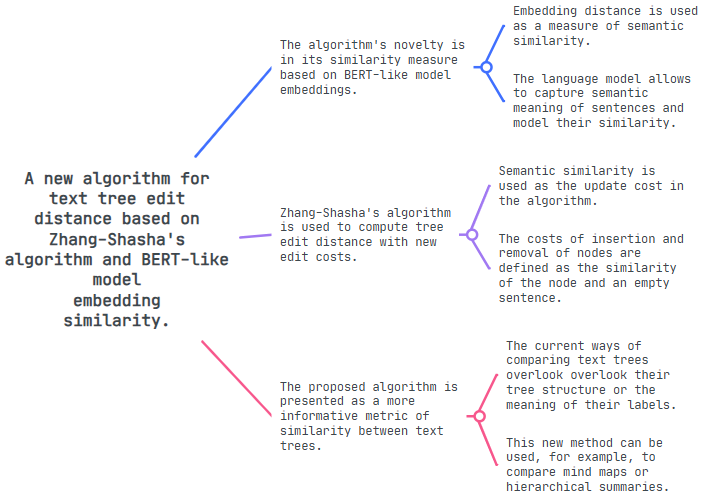
\includegraphics[width=\linewidth]{img/map_example.png}
        \caption{Пример иерархической сводки по научному исследованию}
        \label{fig:map_example}
    \end{figure}
\end{columns}

\end{frame}

%%%%%%%%%%%%%%%%%%%%%%%%%%%%%%%%%%%%%%%%%%%%%%%%%%%%%%%%%%%%%%%%%%%%%%%%%%

\begin{frame}{Постановка задачи иерархической суммаризации}

\begin{itemize}
    \item Пусть $\mathcal{S}$~--- множество возможных фрагментов текста. \item Текстовое дерево~--- дерево $T = (V, E)$, где $E \subset V^2$ и для каждого $v\in V$ определен текст $s(v)\in\mathcal{S}$. 
    \item $\mathcal{T}$~--- множество рассматриваемых текстовых деревьев.
    \item $\rho: T^2\rightarrow\R^+$~--- числовая метрика различия текстовых деревьев.
    \item Задача: найти отображение $f: D\mapsto T$, строящее иерархическую сводку $T\in\mathcal{T}$ по документу $D$, минимизирующее ее отличие от авторской сводки $T^*$:
    $$
    \rho(f(D), T^*)\longrightarrow\min_f.
    $$
\end{itemize}

\end{frame}

%%%%%%%%%%%%%%%%%%%%%%%%%%%%%%%%%%%%%%%%%%%%%%%%%%%%%%%%%%%%%%%%%%%%%%%%%%

\begin{frame}{Требования к метрике сходства текстовых деревьев}

Пусть $T, T' \in\mathcal{T}$. Зададим следующие требования к метрике $\rho$ на множестве $\mathcal{T}$:
\begin{enumerate}
    \item Симметричность: $\rho(T, T') = \rho(T', T)$.
    \item Равенство нулю в случае равенства аргументов: $\rho(T, T) = 0$.  
    \item $\rho$ удовлетворяет неравенству треугольника: 
    \begin{equation} \label{metric_requirement_6}
        \forall T, T', T''\in\mathcal{T}\quad \rho(T,T'')\leq\rho(T,T')+\rho(T',T'').
    \end{equation}
    \item Существует некоторая неубывающая функция $f: \R^+ \rightarrow \R^+$, такая что:
    \begin{enumerate}
        \item Если $T'$ получено из $T$ добавлением в $T$ вершины $v$, то $\rho(T, T') = f(r(v))$;
        \item Если $T'$ получено из $T$ удалением из $T$ вершины $v$, то $\rho(T, T') = f(r(v))$;
        \item Если $T'$ получено из $T$ заменой вершины $v$ на $v'$, то $\rho(T, T')= f(r(v, v'))$.
    \end{enumerate}
\end{enumerate}

\end{frame}

%%%%%%%%%%%%%%%%%%%%%%%%%%%%%%%%%%%%%%%%%%%%%%%%%%%%%%%%%%%%%%%%%%%%%%%%%%

\begin{frame}{Предлагаемая метрика~--- \textit{TTED}}

\begin{itemize}
    \item \textit{\textbf{TTED} (text tree edit distance)}~--- расстояние редактирования\footnote{\textit{Zhang Kaizhong, Statman Richard, Shasha Dennis.} On the Editing Distance Between Unordered Labeled Trees}, стоимости операций редактирования в котором определяются заданной мерой семантического расстояния между текстами в вершинах. 
    \item В качестве метрики семантического расстояния можно применить языковую модель $\text{LM}: S \rightarrow \R^n$ и определить для $s, s'\in\mathcal{S}$ семантическое расстояние как $r(s, s') = \rho_n(\text{LM}(s), \text{LM}(s'))$, где $\rho_n$~--- функция расстояния в $\R^n$.
\end{itemize}
\begin{block}{Используемые эвристики:}
    \begin{itemize}
        \item Использование родительских вершин в качестве \textbf{контекста} для текстов в дочерних.
        \item \textbf{Предварительное вычисление} эмбеддингов и попарных расстояний для всех текстов в вершинах.
    \end{itemize}    
\end{block}

\end{frame}

%%%%%%%%%%%%%%%%%%%%%%%%%%%%%%%%%%%%%%%%%%%%%%%%%%%%%%%%%%%%%%%%%%%%%%%%%%

\begin{frame}{Базовый метод}

\begin{itemize}
\item Для сравнения используется оценка сходства текстовых деревьев из работы \textit{Zhang et al., 2024}\footnote{\textit{Zhang Zhuowei, Hu Mengting, Bai Yinhao, and Zhang Zhen.} Coreference Graph Guidance for Mind-Map Generation}. Для текстовых деревьев $T=(V, E)$ и $T'=(V',E')$ она определяется как:
$$
\text{Sim}(T, T') = \min\limits_{P\subset E\times E'} \sum\limits_{(e, e')\in P}\sum\limits_{i=0,1}\text{ROUGE}(e_i, e'_i).
$$
где $P$~--- однозначное сопоставление ребер $T$ ребрам $T'$ (оптимальное ищется жадных алгоритмом), ROUGE$(v, v')$~--- усредненная оценка ROUGE-1, ROUGE-2 и ROUGE-L сходства $s(v)$ и $s(v')$.
\item В экспериментах для единообразия в качестве оценки расстояния используется $\rho(T, T') = \text{Sim}^{\max} - \text{Sim}(T, T')$, где $\text{Sim}^{\max} = \text{Sim}(T, T)$.
\end{itemize}

\end{frame}

%%%%%%%%%%%%%%%%%%%%%%%%%%%%%%%%%%%%%%%%%%%%%%%%%%%%%%%%%%%%%%%%%%%%%%%%%%

\begin{frame}{Критерии качества метрики}

Пусть для $T\in\mathcal{T}$:
\begin{itemize}
    \item $P(T)$ множество деревьев~--- парафразов $T$;
    \item $S(T)$~--- множество деревьев~--- реструктуризаций $T$; 
    \item $M(T)$~--- набор деревьев с такой же структурой, как у $T$, но с разной семантикой: $M(T) = \mathcal{T}_{\sim T} \setminus P(T)$.
\end{itemize}
Задача оптимизации:
$$
R_S(\rho) \longrightarrow \min_\rho, \quad  R_M(\rho) \longrightarrow \min_\rho,
$$
где
$$
R_S(\rho) = \E_{T\sim \mathcal{T}}[r_S(\rho, T)], \quad R_M(\rho) = \E_{T\sim \mathcal{T}}[r_M(\rho, T)],
$$
$$
r_S(\rho, T) = \E_{T'\sim P(T), \ T''\sim S(T)} \left[\frac{\rho(T, T')}{\rho(T, T'')}\right],
$$
$$
r_M(\rho, T) = \E_{T'\sim P(T), \ T'''\sim M(T)} \left[\frac{\rho(T, T')}{\rho(T, T''')}\right].
$$

\end{frame}

%%%%%%%%%%%%%%%%%%%%%%%%%%%%%%%%%%%%%%%%%%%%%%%%%%%%%%%%%%%%%%%%%%%%%%%%%%%

\begin{frame}{Оценка коэффициентов качества по выборке}

Рассмотрим случайную выборку текстовых деревьев $\mathcal{D} = \{T, T'_1, \dots, T'_p, T''_1, \dots, T''_s, T'''_1, \dots, T'''_m\}$, где $T\sim \mathcal{T}$, $T'_i\sim P(T)$, $T''_j\sim S(T)$, $T'''_k\sim M(T)$. Введем следующие оценки на $R_S(\rho)$ и $R_M(\rho)$ по $\mathcal{D}$:
$$
R^\mathcal{D}_S(\rho) = \frac{1}{sp}\sum\limits_{i=1}^p\sum\limits_{j=1}^s\frac{\rho(T, T'_i)}{\rho(T, T_j'')},
\quad R^\mathcal{D}_S(\rho) = \frac{1}{mp}\sum\limits_{i=1}^p\sum\limits_{k=1}^m\frac{\rho(T, T'_i)}{\rho(T, T_k''')}.
$$
\begin{Th}[Соболевский, 2025]
    Пусть для заданного класса текстовых деревьев $\mathcal{T}$ и метрики $\rho: \mathcal{T}\times\mathcal{T}\longrightarrow [0, +\infty)$ существуют конечные $R_S(\rho)$ и $R_M(\rho)$. Тогда $R_S^\mathcal{D}(\rho)$ и $R_M^\mathcal{D}(\rho)$ являются несмещенными оценками $R_S(\rho)$ и $R_M(\rho)$ соответственно по случайной выборке $\mathcal{D}$:
    $$
    \E_\mathcal{D}[R_S^\mathcal{D}(\rho)] = R_S(\rho), \quad \E_\mathcal{D}[R_M^\mathcal{D}(\rho)] = R_M(\rho).
    $$
\end{Th}
    
\end{frame}

%%%%%%%%%%%%%%%%%%%%%%%%%%%%%%%%%%%%%%%%%%%%%%%%%%%%%%%%%%%%%%%%%%%%%%%%%%%

\begin{frame}{Многокритериальное сравнение текстовых деревьев}

Для сравнения текстовых деревьев по различным аспектам сходства применимы следующие метрики:
\begin{itemize}
    \item \textbf{Семантическое сходство:} сравнение текстов из вершин деревьев как линейных с помощью \textit{BERTScore}\footnote{\textit{Zhang Tianyi, Kishore Varsha, Wu Felix, Weinberger Kilian Q, Artzi Yoav.} BERTScore: Evaluating text generation with BERT};
    \item \textbf{Структурные различия:} сравнение деревьев без разметки с помощью \textit{расстояния редактирования} \textit{(TED)};
    \item \textbf{Сходство ранжирования} предложений в иерархии: сопоставление предложений в вершинах по семантической близости и сравнение ранжирования с помощью \textit{коэффициента корреляции Спирмена}\footnote{\textit{Spearman Charles.} The Proof and Measurement of Association between Two Thing} ($r_S$).
\end{itemize}
    
\end{frame}

%%%%%%%%%%%%%%%%%%%%%%%%%%%%%%%%%%%%%%%%%%%%%%%%%%%%%%%%%%%%%%%%%%%%%%%%%%%

\begin{frame}{Тестирование метрик~--- постановка эксперимента}

Для оценки семантической близости в TTED использовался ряд языковых моделей из библиотеки \texttt{sentence-transformers}\footnote{\texttt{https://sbert.net/}}. 

Эксперименты~--- вычисление расстояний на выборке, состоящей из:
\begin{enumerate}
    \item Основного дерева $T$, с которым сравнивались остальные;
    \item Парафразов $T$ (подвыборка \texttt{paraphrase});
    \item Реструктуризаций $T$ (подвыборка \texttt{restructure});
    \item Деревьев, отличных от $T$ только по смыслу (подвыборка \texttt{meaning}).
\end{enumerate}
\textbf{Цель эксперимента}~--- найти среди предложенных такую метрику $\rho$, для которой будут минимальными оценки $R_S^\mathcal{D}(\rho)$ и $R_M^\mathcal{D}(\rho)$.

\end{frame}

%%%%%%%%%%%%%%%%%%%%%%%%%%%%%%%%%%%%%%%%%%%%%%%%%%%%%%%%%%%%%%%%%%%%%%%%%%

\begin{frame}{Тестирование метрик~--- результаты}

\begin{columns}

\column{0.5\textwidth}
\begin{figure}
    \centering
    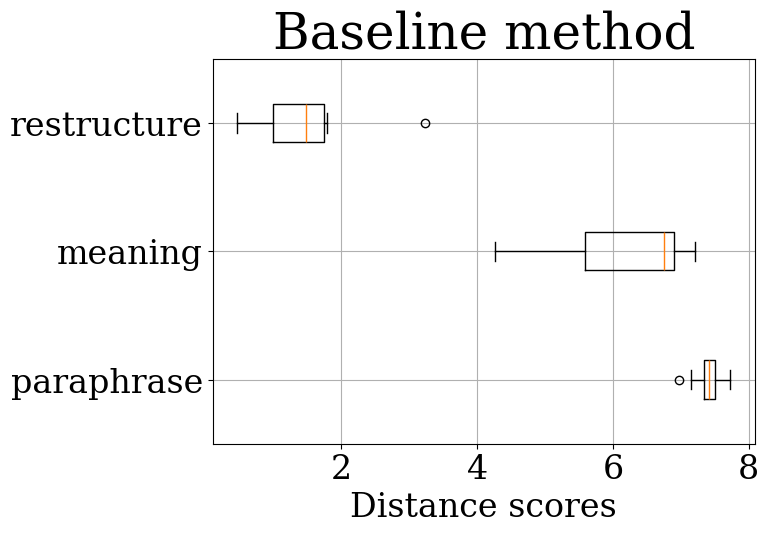
\includegraphics[width=\textwidth]{img/baseline_results.png}
    \caption{Оценки базового метода}
    \label{fig:baseline}
\end{figure}

\column{0.5\textwidth}
\begin{figure}
    \centering
    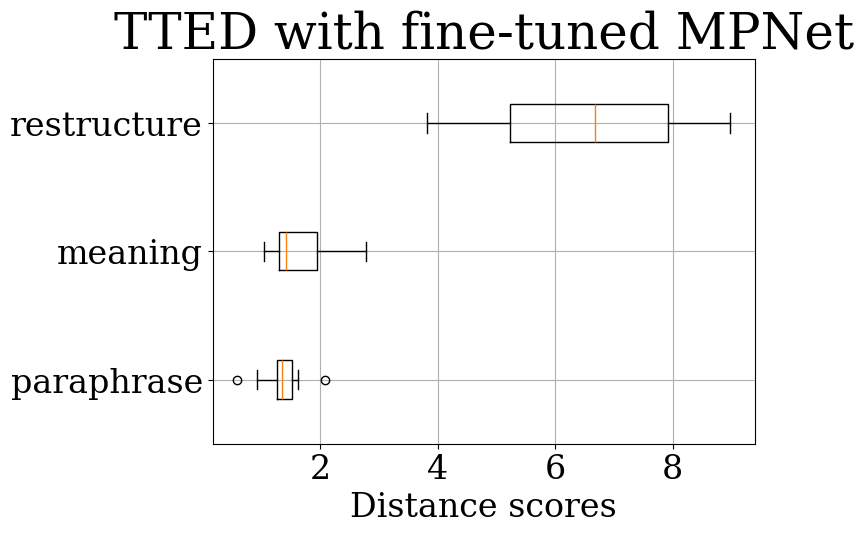
\includegraphics[width=\textwidth]{img/paraphrase_mpnet_results.png}
    \caption{Оценки нашего метода}
    \label{fig:results}
\end{figure}

\end{columns}

\begin{table}[h]
    \centering
    \begin{tabular}{c|c|c}
        Модель & $R_S^\mathcal{D}(\rho)$ & $R_M^\mathcal{D}(\rho)$ \\ \hline
        Baseline & 6,29$\pm$3,58 & 1,22$\pm$0,24 \\ \hline
        DistilRoBERTa & 0,38$\pm$0,11 & 0,89$\pm$0,28 \\ \hline
        SPECTER & 0,41$\pm$0,14 & 0,92$\pm$0,27 \\ \hline
        MPNet & 0,27$\pm$0,07 & 1,07$\pm$0,59 \\ \hline
        Fine-tuned MPNet & \textbf{0,21$\pm$0,05} & \textbf{0,88$\pm$0,37}
    \end{tabular}
    \caption{Средние оценки расстояния с помощью разных языковых моделей}
    \label{tab:model_results}
\end{table}

\end{frame}

%%%%%%%%%%%%%%%%%%%%%%%%%%%%%%%%%%%%%%%%%%%%%%%%%%%%%%%%%%%%%%%%%%%%%%%%%%

\begin{frame}{Тестирование БЯМ~--- постановка эксперимента}

Используемая для тестирования БЯМ~--- модель \texttt{mistral-large-latest} из библиотеки \texttt{langchain-mistralai}\footnote{\texttt{https://python.langchain.com/docs/integrations/providers/mistralai/}}.

Исследованные методы генерации иерархических сводок:
\begin{enumerate}
    \item \textbf{Прямой промптинг} (direct prompting) модели созданными вручную запросами;
    \item \textbf{Оптимизация запросов} (prompt optimization) с помощью библиотеки \texttt{langmem}\footnote{\texttt{https://langchain-ai.github.io/langmem/}} с использованием многокритериальной оценки генерации с помощью человеческих запросов;
    \item \textbf{Последовательный промптинг} (sequential prompting) модели с выбором пользователем генерируемых вершин дерева.
\end{enumerate}
Метрики сходства по различным аспектам~--- BERTScore, TED, $r_s$, а также единая метрика TTED. 

\end{frame}

%%%%%%%%%%%%%%%%%%%%%%%%%%%%%%%%%%%%%%%%%%%%%%%%%%%%%%%%%%%%%%%%%%%%%%%%%%

\begin{frame}{Тестирование БЯМ~--- результаты}

\begin{table}[]
    \centering
    \begin{tabular}{c|c|c|c}
        Метод & BERTScore & TED & TTED \\ \hline
        Direct prompting & 0,41 & 11,0 & 14,13 \\ \hline
        Prompt optimization & 0,72 & 4,0 & 7,26 \\ \hline
        Sequential prompting & \textbf{0,78*} & \textbf{0,0*} & \textbf{3,35*} \\
    \end{tabular}
    \caption{Результаты тестирования БЯМ для иерархической суммаризации}
    \label{tab:llm_tests}
\end{table}

\textit{*При оптимальном сценарии взаимодействия пользователя с системой.}

\end{frame}

%%%%%%%%%%%%%%%%%%%%%%%%%%%%%%%%%%%%%%%%%%%%%%%%%%%%%%%%%%%%%%%%%%%%%%%%%%

\begin{frame}{Заключение}
    \begin{block}{Положения, выносимые на защиту}
        \begin{itemize}
            \item Введен новый коэффициент качества метрик на множестве текстовых деревьев и предложена несмещенная оценка данного коэффициента по случайной выборке текстовых деревьев.
            \item Разработан новый алгоритм оценки расстояния между текстовыми деревьями, лучше отражающий значимые отличия текстовых деревьев в терминах введенного коэффициента качества, чем используемые до этого методы.
            \item Проведено многокритериальное исследование методов иерархической суммаризации при помощи БЯМ с использованием предложенных новых методов сравнения с экспертными сводками.
        \end{itemize}
    \end{block}
\end{frame}

%%%%%%%%%%%%%%%%%%%%%%%%%%%%%%%%%%%%%%%%%%%%%

\begin{frame}{Литература}

\begin{itemize}
    \item \textit{Zhang Z., Hu M., et al.} Coreference Graph Guidance for Mind-Map Generation // Proceedings of the AAAI Conference on Artificial Intelligence. — 2024. — Vol. 38. — P. 19623–19631.
    \item \textit{Zhang K., Statman R., Shasha D.} On the editing distance between unordered labeled trees. // Information processing letters. 1992 May 25; 42(3): 133-9.
    \item \textit{Vrbanec T., Meštrović A.} Comparison study of unsupervised paraphrase detection: Deep learning — The key for semantic similarity detection. // Expert systems. 2023 Nov; 40(9): e13386.
\end{itemize}

\end{frame}

%%%%%%%%%%%%%%%%%%%%%%%%%%%%%%%%%%%%%%%%%%%%%%%%%%%%%%%%%%%%%%%%%%%%%%%%%%

\end{document} 